\documentclass[11pt,xcolor=svgnames]{beamer}
\usepackage{dsfont,natbib,setspace,changepage,multirow}
\mode<presentation>

% replaces beamer foot with simple page number
\setbeamertemplate{navigation symbols}{}
\setbeamerfont{frametitle}{series=\bfseries,size=\normalsize}
\setbeamercolor{frametitle}{fg=Black}

\setbeamertemplate{footline}{
   \raisebox{5pt}{\makebox[\paperwidth]{\hfill\makebox[20pt]{\color{gray}\scriptsize\insertframenumber}}}}

\usepackage{algorithm}
\usepackage{algorithmic}

% colors
\newcommand{\theme}{\color{DarkBlue}}
\newcommand{\bk}{\color{black}}
\newcommand{\rd}{\color{red}}
\newcommand{\fg}{\color{ForestGreen}}
\newcommand{\bl}{\color{blue}}
\newcommand{\gr}{\color{black!50}}
\newcommand{\sg}{\color{DarkSlateGray}}
\newcommand{\nv}{\color{Navy}}
\setbeamercolor{itemize item}{fg=gray}

% common math markups
\newcommand{\bs}[1]{\boldsymbol{#1}}
\newcommand{\mc}[1]{\mathcal{#1}}
\newcommand{\mr}[1]{\mathrm{#1}}
\newcommand{\bm}[1]{\mathbf{#1}}
\newcommand{\ds}[1]{\mathds{#1}}
\newcommand{\indep}{\perp\!\!\!\perp}
\def\plus{\texttt{+}}
\def\minus{\texttt{-}}

% spacing and style shorthand
\setstretch{1.1}

\begin{document}

\setcounter{page}{0}
{ 
\begin{frame}[plain]
\begin{center}

{\bf \LARGE \theme Regularized Estimation of \\\vskip .25cm Player Performance}
\end{center}

\vskip 1cm
~~~~~~~~{\bf Bobby Gramacy}, Chicago Booth
\vskip .1cm
~~~~~~~~{\bf Matt Taddy},  Microsoft Research and Chicago Booth~~~~
%{\gr \texttt{faculty.chicagobooth.edu/matt.taddy/research}}

\vskip .1cm
{\color{black!70} ~~~~~~~~~~~with  Sen Tian (NYU) and Shane Jenson (Wharton)}


\end{frame} }

\begin{frame}
{Plus-Minus}

PM is a running count of, for every goal, a +1 for those on \\the scoring team and -1 for those on the team scored upon.

\vskip .25cm
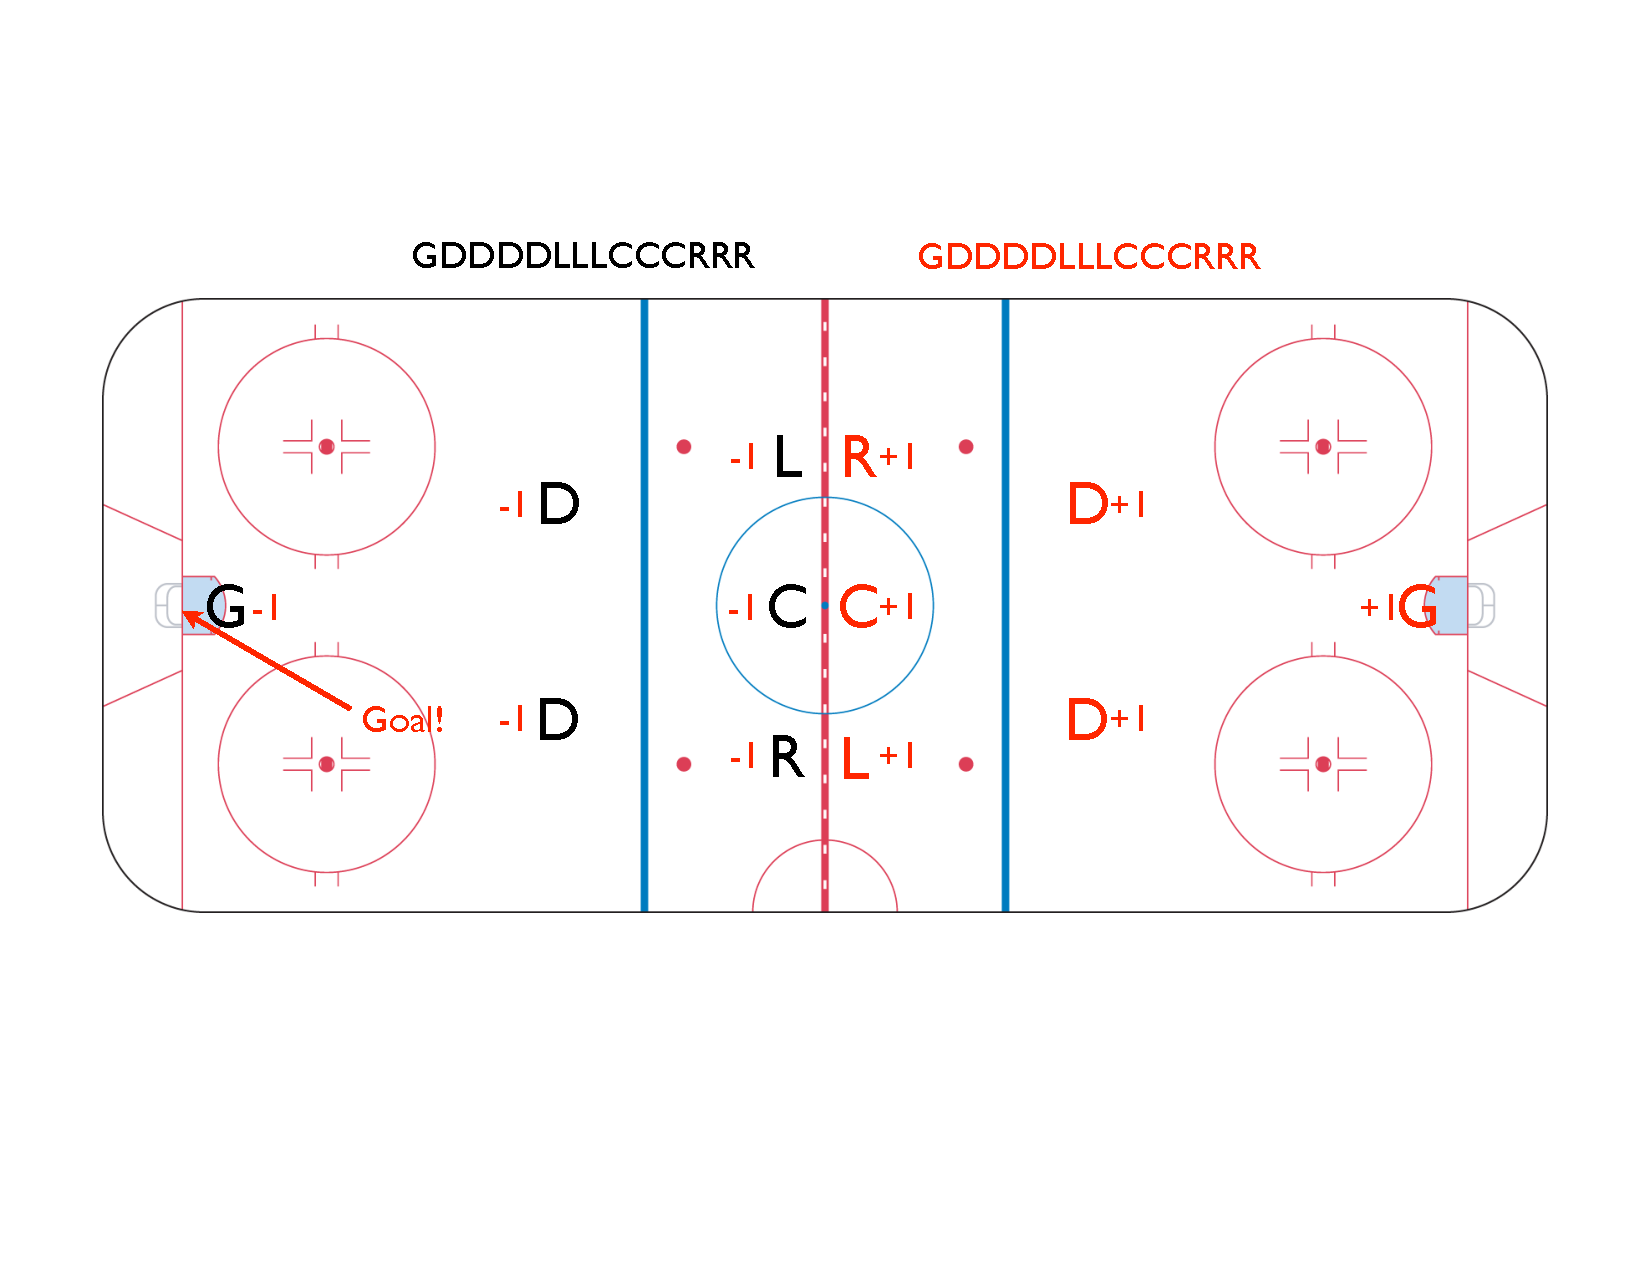
\includegraphics[width=\textwidth]{figures/rink_goal.pdf}

It doesn't quite measure player quality, as we haven't controlled for the effects of teammate and opponent quality (or anything else).

\end{frame}

\begin{frame}
{A Regression version of PM}

Set up a `response' variable:\\
~~~~ $y_i = +1$ for a \textit{home} team goal, \\
~~~~~$y_i = -1$ for an \textit{away} team goal.

\vskip .25cm
We're interested in how individual players affect
\[
{\theme q_i =
\mathrm{p}(y_i = 1) =  \mathrm{p}(\text{home~team~scored~goal}~i)}
\]

The standard model for such problems is logistic regression, say
\[
\log\left[\frac{q_{i}}{1-q_{i}}\right] = \alpha + \beta_{HG} + \beta_{HD} ... +\beta_{HR} - \beta_{AG} - ... - \beta_{AR}
\]
where $\beta_{HG}$ is Home-Goalie and $\beta_{AR}$ is Away-Right-wing, etc. 

\vskip .25cm\gr
Then, for player $j$ and given a goal was scored, $e^\beta_j$ is the multiplier\\ on odds that it was scored by his team if he's on the ice. 
\end{frame}

\begin{frame}

We actually use a larger regression model:
\[\theme 
\log\left[\frac{q_{i}}{1-q_{i}}\right] = \alpha + \mathbf{u}_i'\boldsymbol{\gamma} +
\mathbf{v}_i'\boldsymbol{\varphi} + \mathbf{x}_i'\boldsymbol{\beta}_0 {\gr +
(\mathbf{x}_i\circ\mathbf{s}_i)'(\boldsymbol{\beta}_s + p_i \boldsymbol{\beta}_{p})}
\]
where
\begin{itemize}
\item $\mathbf{u}_i$ holds indicators for each team-season,
\item $\mathbf{v}_i$ holds indicators for various special-teams scenarios,
\item 
$\mathbf{x}_i$ contains player-presence indicator,
\end{itemize}
All of these indicators are +1 for home and -1 for away.

\vskip .25cm
Then $\beta_j$ measures player effect after {\theme controlling} for team strength (e.g., coach or schedule) and on-ice scenarios (e.g., PP or PK).


\vskip .25cm {\gr We also allow deviations in the player effects for specific seasons ($s_{it}$) and in the playoffs ($p_{it}$), but these are seldom `significant'.}

\vskip -.5cm
\end{frame}

\begin{frame}
{Regularization}

Instead of minimizing deviance, we minimize deviance \\{\it plus penalty $\lambda|\beta_j|$ on the size of each $\beta_j$ estimates}.

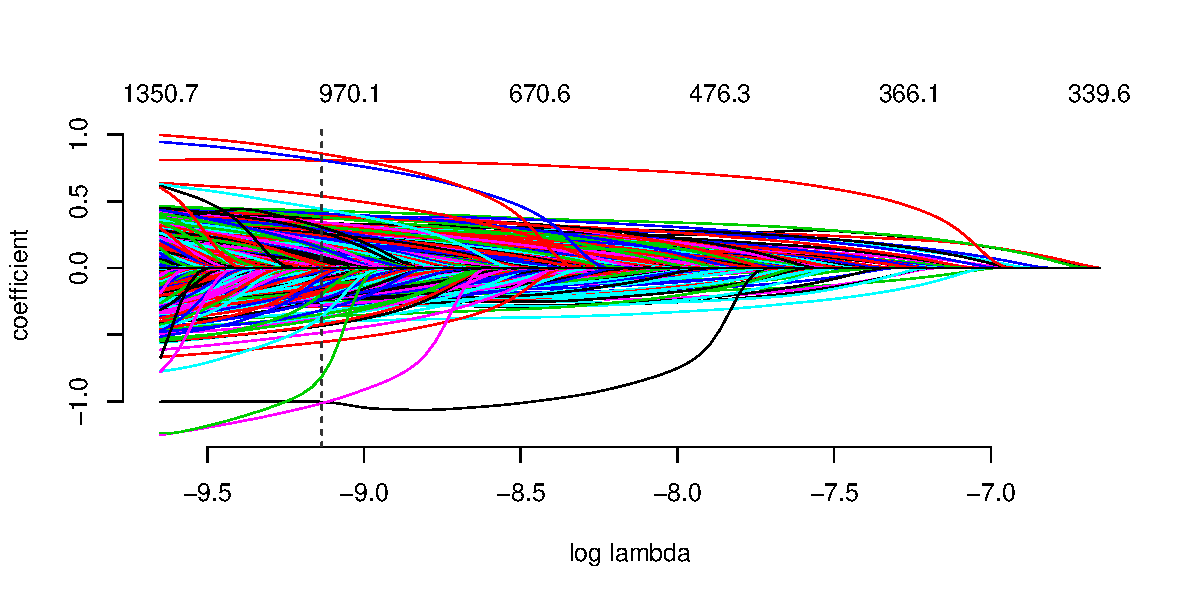
\includegraphics[width=\textwidth]{figures/pathplot.pdf}

Enumerate a `path' of models for different $\lambda$, and use the one that predicts best out-of-sample. {\theme This is how modern stats/ML works.}

\end{frame}
\end{document}